\chapter{Visão}

O sistema de visão, desenvolvido na \textit{CMUCam3}, é responsável principalmente por identificar e localizar o objeto a ser procurado no seu campo de visão, identificar objetos de interesse para serem utilizados na navegação, e identificar obstáculos. Ele também tem a função auxiliar de corrigir desvios na movimentação do robô. De forma a resolver esses problemas, diversas funcionalidades apresentadas pela \textit{CMUcam3} são utilizadas. Diversos exemplos e projetos já existentes também são aproveitados como referência.

\section{Identificação de objetos de interesse}

Uma das principais funções do sistema de visão é localizar, caso se encontre dentro de seu campo de visão, o objeto a ser procurado pelo robô. Como este é simples e possui uma única cor, de destaque, que não existe no ambiente proposto (e é improvável de se encontrar em um ambiente genérico) o mapa de cores obtido com a \textit{CMUcam} pode ser utilizado para localizar o objeto na imagem, aliado a uma ferramenta de reconhecimento de forma.

O sistema também deve localizar, dentro de seu campo de visão, objetos que se destaquem, para serem utilizados pelo sistema de navegação, de forma a identiicar a posição atual. Para a identificação desses objetos, ou pontos de interesse, as características de cor e forma também podem ser utilizadas. Técnicas adicionais para tornar o reconhecimento tolerável à rotação tridimensional não são necessárias, devido às informações obtidas pela bússola.

\section{Identificação de obstáculos}

Obstáculos podem ser identificados, na imagem, através do histograma da imagem obtida, ou então por detecção de bordas. A primeira abordagem é preferível por auxiliar a identificar as áreas (chão) por onde o robô pode se locomover, ao invés dos limites entre o chão e os obstáculos. A \ref{vis_fig01} apresenta algumas imagens exemplo obtidas no site da \textit{CMUcam3}.

\begin{figure}[h!]
    \center
    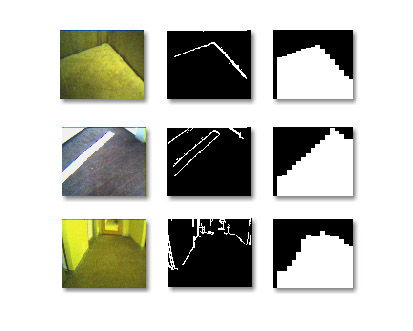
\includegraphics[scale=1]{imagens/polly_sample.jpg}
    \caption{Histograma e Detecção de Bordas de algumas imagens exemplo}
    \label{vis_fig01}
\end{figure}

\section{Correção de desvios}

De forma a corrigir eventuais desvios na movimentação do robô, causados por uma diferença de rotação entre as duas rodas, o sistema também deve identificar, na imagem, através da detecção de bordas e do mapa de cores, alguns objetos ou bordas de destaque, e caso saiam muito do lugar esperado para eles, corrigir sua rota.
